%# -*- coding: utf-8-unix -*-
%%==================================================
\chapter{相对论基础}

本讲义的授课主题,是\gw\DA,共分为两部分,\emph{\gw}与\emph{\DA}。
如果脱离了\gw 的物理图景,而直接空谈\DA,未免空中楼阁。
而在另一方面,引力波又是Einstein广义相对论的直接理论预言,因此,引力波的理论描述,无法跳脱广义相对论的框架。

\begin{figure}[htp]
\centering
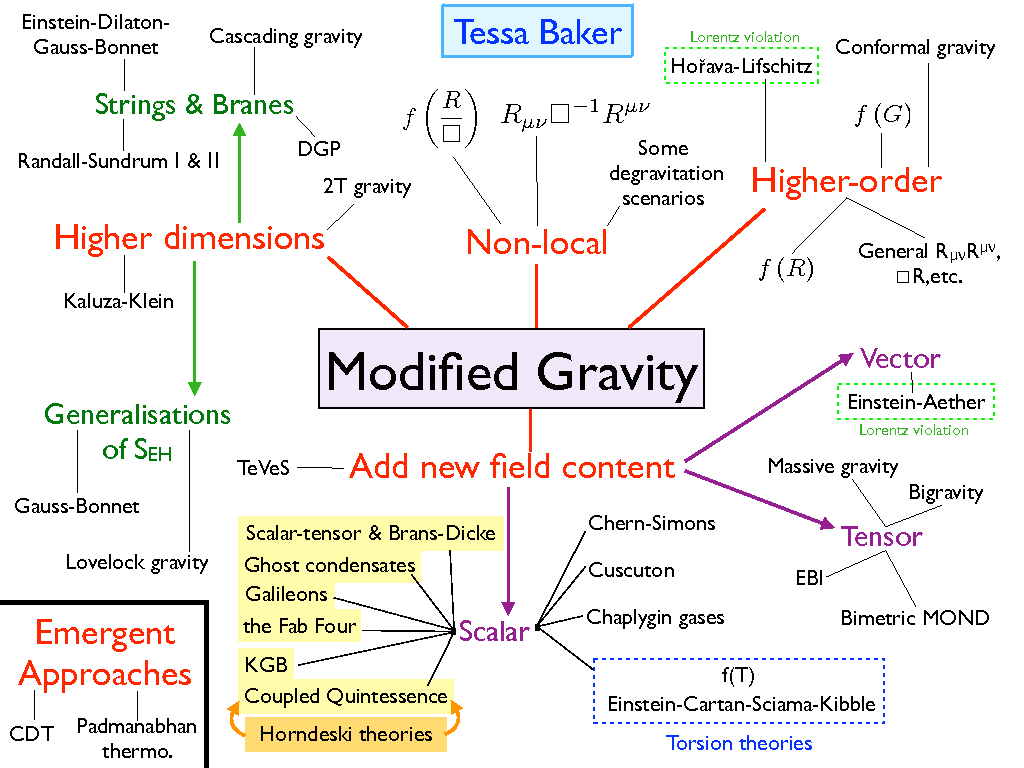
\includegraphics[width=0.7\textwidth]{ModifiedGravity.png}
\bicaption{修改引力理论}
  {Theories of modified gravity. Credit: http://www.cgc-yzu.cn/Upload/research/MG-20240317524.png}
\label{fig:ModGrav}
\end{figure}

从Einstein至今,引力理论已经有了长足的发展,如图\ref{fig:ModGrav}所示,仅基于\GR 基础上发展起来的修改引力理论就已不计其数。
由于和量子力学原理的深刻矛盾,有理由认为Einstein决定论性的的\GR 在某个地方一定背离了引力的物理本质。
然而,时至今日,Einstein昔日基于\GR 所作出的诸多预言,一一被实验所验证;所有可靠的实验检验下,\GR 均可以给出解释——而它通常是最简洁的那个理论。
因此,即使将来的实验证明了\GR 与引力的物理本质之间的偏离,对\GR 的理解依然有着重要的意义。

\section{相对性原理(Principle of relativity)}

\subsection{Galilean相对论}
虽然在20世纪,相对论一次专职Einstein的理论,但是相对性原理(Principle of relativity)的思想在牛顿力学中就有体现,一般认为是Galileo在《关于Ptolemaic和 Copernican两大世界体系的对话》中首先提出的:
\begin{myprop}{}{}
把你和一些朋友关在一条大船的甲板下的主舱里,让你们带着几支苍蝇、蝴蝶和其他小飞虫,舱内放一支大碗,其中有几条鱼,然后,挂上一个水瓶,让水一滴一滴地滴到下面的一个宽口罐里。船停着不动时,你留神观察,小虫都以等速向舱内各方向飞行,鱼向各方向随便游动,水滴滴进下面的罐中。你把任何东西扔给你的朋友时,只要距离相等,向这一方向也不比向另一方向更多用力。你的双脚齐跳,无论向哪个方向跳过的距离都相等。当你仔细观察这些事情之后,再使船以任何速度前进,只要运动是均匀的,也不忽左忽右地摆动,你将发现,所有上述现象都没有丝毫变化,你无法从任何一个现象来确定,船是在运动还是在停着不动。即使船运动得相当快,在跳跃时,你也将和以前一样,你跳向船尾也不会比跳向船头更省力。
\end{myprop}

